\documentclass[10pt,a4paper,twocolumn]{article}
\usepackage[a4paper,top=2.3cm,bottom=1.9cm,left=1.4cm,right=1.4cm,columnsep=0.9cm,headsep=0.5cm]{geometry}

\usepackage{fontspec}
\setmainfont{texgyreheros}[Extension=.otf,UprightFont=*-regular,BoldFont=*-bold,ItalicFont=*-italic,BoldItalicFont=*-bolditalic]
\setsansfont{texgyreheros}[Extension=.otf,UprightFont=*-regular,BoldFont=*-bold,ItalicFont=*-italic,BoldItalicFont=*-bolditalic]

\usepackage[brazil]{babel}
\usepackage{amsmath,amssymb}
\usepackage{graphicx}
\usepackage[table]{xcolor}
\usepackage{tikz}
\usetikzlibrary{arrows.meta,calc,positioning,patterns,angles,quotes,shapes.geometric,decorations.pathreplacing}
\usepackage{pgfplots}
\pgfplotsset{compat=1.18}

\usepackage{fancyhdr,needspace,tabularx,array,enumitem}
\setlength{\columnseprule}{0.4pt}
\setlength{\parindent}{0pt}
\setlength{\parskip}{4.5pt}
\renewcommand{\baselinestretch}{1.05}
\sloppy
\pagestyle{fancy}\fancyhf{}
\renewcommand{\headrulewidth}{0pt}
\newcommand{\faixa}{\colorbox{black}{\makebox[\dimexpr\textwidth-2\fboxsep\relax][l]{\color{white}\bfseries\footnotesize SIMULADO MULTIDISCIPLINAR\hfill 1º DIA | CADERNO 1 | AZUL\quad\thepage}}}
\fancyhead[C]{\faixa}
\fancyfoot[C]{\tiny Material didático elaborado com a skill-enem. Não é material oficial do Inep.}
\fancypagestyle{plain}{\fancyhf{}\fancyhead[C]{\faixa}\fancyfoot[C]{\tiny Material didático elaborado com a skill-enem. Não é material oficial do Inep.}}
\newcommand{\questao}[1]{\needspace{7\baselineskip}\par\vspace{7pt}\noindent{\bfseries\large QUESTÃO #1}\par\vspace{1pt}}
\newcommand{\referencia}[1]{\par\vspace{-2pt}{\raggedleft\scriptsize #1\par}\vspace{2pt}}
\newcommand{\rotulo}[1]{\par{\centering\bfseries\small #1\par}}
\newcommand{\bolinha}[1]{\tikz[baseline=(c.base)]\node[circle,draw,line width=0.5pt,inner sep=0pt,minimum size=1.15em,font=\scriptsize\bfseries](c){#1};}
\newcommand{\alt}[2]{\par\vspace{1.5pt}\noindent\hangindent=1.75em\hangafter=1\makebox[1.75em][l]{\bolinha{#1}}#2\par}
\newenvironment{poema}{\par\begingroup\leftskip=1.2em\parskip=0pt\raggedright}{\par\endgroup\vspace{3pt}}

\begin{document}
\twocolumn[{\begin{center}{\Large\bfseries Simulado no estilo ENEM — Exemplo}\par\vspace{4pt}
{\small Questões elaboradas pela skill-enem para demonstração (textos elaborados para fins didáticos)}\par\vspace{4pt}
\end{center}
\noindent\fbox{\parbox{\dimexpr\textwidth-2\fboxsep-2\fboxrule\relax}{\footnotesize\textbf{INSTRUÇÕES}\begin{enumerate}[leftmargin=1.4em,itemsep=0pt,topsep=2pt]\item Este caderno contém questões de múltipla escolha com cinco alternativas (A, B, C, D e E), das quais apenas uma é correta.\item Leia atentamente cada questão e marque a alternativa que responde corretamente ao que é pedido.\item Reserve, em média, 3 minutos por questão.\end{enumerate}}}\vspace{8pt}
}]
\questao{01}
\begin{center}\fbox{\parbox{0.92\linewidth}{\centering Biblioteca Municipal @bibliomunicipal

Spoiler: a gente tem MUITO livro que vira série! Antes de maratonar, que tal ler primeiro e depois comparar? Chega aí que a carteirinha sai na hora, é de graça e sem burocracia. Bora?

\#LeiaAntes \#BibliotecaÉPraTodos}}\end{center}
\referencia{Texto elaborado para fins didáticos.}
\par\vspace{2pt}Nesse post, a escolha de um registro informal, com gírias e \emph{hashtags}, tem como objetivo
\alt{A}{substituir o hábito de assistir a séries pela prática regular da leitura.}
\alt{B}{informar os procedimentos necessários para a emissão da carteirinha.}
\alt{C}{criticar a adaptação de obras literárias para plataformas de \emph{streaming}.}
\alt{D}{aproximar a biblioteca do público jovem, usando a linguagem das redes sociais.}
\alt{E}{divulgar o lançamento de uma série inspirada no acervo da biblioteca.}
\questao{02}
Em uma tarde de verão, estudantes mediram a temperatura do ar em cinco pontos de uma mesma cidade, no mesmo horário. Os resultados estão no gráfico.
\begin{center}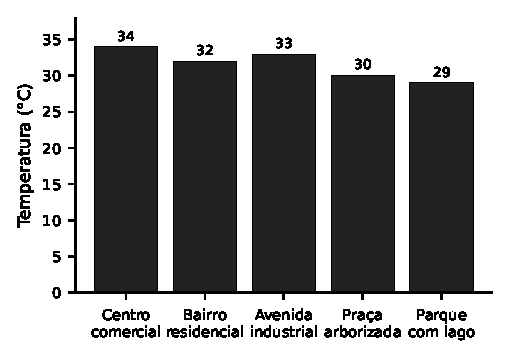
\includegraphics[width=0.95\linewidth]{figuras/fig01.pdf}\end{center}
O centro comercial tem ruas asfaltadas, edifícios próximos uns dos outros e poucas árvores; o parque tem solo coberto por vegetação e um lago.
\referencia{Texto elaborado para fins didáticos.}
\par\vspace{2pt}A diferença de temperatura entre o centro comercial e o parque está associada à
\alt{A}{ocorrência de inversão térmica, que retém o ar quente junto à superfície urbana.}
\alt{B}{intensificação do efeito estufa, que eleva a temperatura média do planeta.}
\alt{C}{redução da camada de ozônio, que aumenta a radiação nas áreas centrais.}
\alt{D}{elevação da umidade do ar, que dificulta a dispersão do calor no centro.}
\alt{E}{substituição da cobertura vegetal por superfícies que absorvem e irradiam calor.}
\questao{03}
Uma família vai instalar um chuveiro elétrico com as especificações 6 600 W – 220 V. O eletricista explica que o circuito do chuveiro deve ser protegido por um disjuntor de corrente nominal maior que a corrente de funcionamento do aparelho; caso contrário, ele desarmará durante o banho. Por economia e segurança, deve-se escolher o disjuntor de \textbf{menor} corrente nominal que atenda a essa condição. A loja dispõe dos modelos indicados no quadro.
\begin{center}\footnotesize\renewcommand{\arraystretch}{1.25}
\begin{tabularx}{1.0\linewidth}{|>{\centering\arraybackslash}X|>{\centering\arraybackslash}X|>{\centering\arraybackslash}X|>{\centering\arraybackslash}X|>{\centering\arraybackslash}X|>{\centering\arraybackslash}X|}\hline
\cellcolor{gray!20}\textbf{Modelo} & \cellcolor{gray!20}\textbf{I} & \cellcolor{gray!20}\textbf{II} & \cellcolor{gray!20}\textbf{III} & \cellcolor{gray!20}\textbf{IV} & \cellcolor{gray!20}\textbf{V}\\\hline
Corrente nominal (A) & 25 & 32 & 40 & 50 & 63\\\hline
\end{tabularx}\end{center}
\referencia{Texto elaborado para fins didáticos.}
\par\vspace{2pt}Considerando que a potência elétrica é dada por $P = U \cdot i$, qual modelo de disjuntor deve ser instalado?
\alt{A}{I}
\alt{B}{II}
\alt{C}{III}
\alt{D}{IV}
\alt{E}{V}
\questao{04}
Um supermercado vende arroz em pacotes de 5 kg, por R\$ 27,50, e em pacotes de 2 kg, por R\$ 11,60. Nesta semana, há uma promoção apenas para os pacotes de 2 kg: na compra de 3 desses pacotes, o cliente paga o preço de 2. Uma cozinha comunitária precisa comprar exatamente 12 kg de arroz e quer gastar o mínimo possível.
\referencia{Texto elaborado para fins didáticos.}
\par\vspace{2pt}Qual é o menor valor, em real, que essa cozinha pagará pelo arroz?
\alt{A}{23,20}
\alt{B}{46,40}
\alt{C}{66,00}
\alt{D}{66,60}
\alt{E}{69,60}
\questao{05}
Durante uma estiagem, a companhia de abastecimento de um município registrou diariamente o nível de um reservatório, em porcentagem da capacidade total. O gráfico apresenta os registros dos sete primeiros dias de observação.
\begin{center}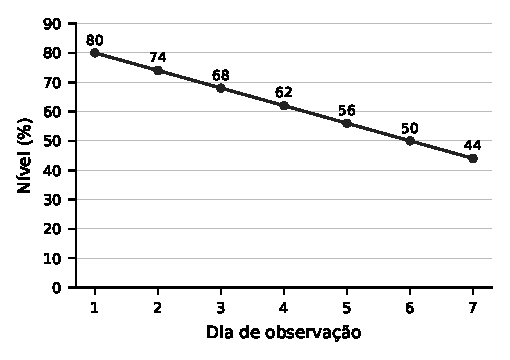
\includegraphics[width=0.95\linewidth]{figuras/fig02.pdf}\end{center}
A companhia decretará racionamento quando o nível atingir 20\% da capacidade.
\referencia{Texto elaborado para fins didáticos.}
\par\vspace{2pt}Mantida a tendência observada, o racionamento será decretado no dia de observação de número
\alt{A}{9}
\alt{B}{10}
\alt{C}{11}
\alt{D}{12}
\alt{E}{14}
\questao{06}
Uma escola vai construir uma rampa de acesso para vencer um desnível de 0,6 m entre a calçada e a entrada do prédio. As normas de acessibilidade adotadas pela prefeitura determinam que a inclinação da rampa, dada pela razão entre a altura vencida e o comprimento horizontal, expressa em porcentagem, não pode ultrapassar 8\%. O esquema representa a rampa vista de lado.
\begin{center}\begin{tikzpicture}[scale=0.85,font=\footnotesize]\fill[gray!15] (0,0)--(7,0)--(7,1.2)--cycle;\draw[thick] (0,0)--(7,0)--(7,1.2)--cycle;\draw (6.7,0)--(6.7,0.3)--(7,0.3);\draw[<->] (7.4,0)--(7.4,1.2) node[midway,right]{0,6 m};\draw[<->] (0,-0.35)--(7,-0.35) node[midway,below]{comprimento horizontal};\node at (3.2,1.0) {rampa};\draw (1.2,0) arc (0:9.7:1.2);\end{tikzpicture}\end{center}
\referencia{Texto elaborado para fins didáticos.}
\par\vspace{2pt}Para atender às normas, o comprimento horizontal mínimo da rampa, em metro, deve ser
\alt{A}{4,8}
\alt{B}{6,0}
\alt{C}{7,5}
\alt{D}{8,0}
\alt{E}{13,3}
\onecolumn
\section*{Gabarito}
\begin{center}\begin{tabular}{|c|c|c|c|c|c|}\hline\textbf{01} & \textbf{02} & \textbf{03} & \textbf{04} & \textbf{05} & \textbf{06}\\
D & E & B & B & C & C\\\hline\end{tabular}\end{center}
\section*{Gabarito comentado e ficha técnica}
\needspace{6\baselineskip}\subsection*{Questão 01 — gabarito D}
{\small Área: LC \textbullet{} Competência: 7 \textbullet{} Habilidade: LC-H23 \textbullet{} Eixo cognitivo: CA \textbullet{} Objeto de conhecimento: Gêneros digitais: recursos linguísticos e interlocutores \textbullet{} Dificuldade estimada: fácil \textbullet{} b estimado (escala 500/100): 470 \textbullet{} Tempo estimado: 2 min}\par
\begin{itemize}[leftmargin=1.5em,itemsep=1pt]
\item \textbf{A:} Extrapola o texto: o post propõe ler antes e comparar, e não abandonar as séries.
\item \textbf{B:} Toma um detalhe (a carteirinha) pelo objetivo da escolha do registro; a informação sobre a carteirinha é secundária.
\item \textbf{C:} Inverte a atitude do texto, que valoriza as adaptações ao sugerir a comparação.
\item \textbf{D (correta):} O registro informal, as gírias ("Chega aí", "Bora?") e as hashtags reproduzem a linguagem das redes sociais para criar proximidade com o público jovem, alvo do convite.
\item \textbf{E:} Introduz um fato ausente do post: não há lançamento de série mencionado.
\end{itemize}
\needspace{6\baselineskip}\subsection*{Questão 02 — gabarito E}
{\small Área: CH \textbullet{} Competência: 6 \textbullet{} Habilidade: CH-H27 \textbullet{} Eixo cognitivo: CF \textbullet{} Objeto de conhecimento: Questões ambientais contemporâneas: ilhas de calor \textbullet{} Dificuldade estimada: médio \textbullet{} b estimado (escala 500/100): 560 \textbullet{} Tempo estimado: 3 min}\par
\begin{itemize}[leftmargin=1.5em,itemsep=1pt]
\item \textbf{A:} Confunde com inversão térmica, fenômeno típico de dias frios que retém poluentes, e não explica diferenças entre bairros no mesmo horário.
\item \textbf{B:} Troca a escala local pela global: o efeito estufa não explica diferenças de 5 °C entre pontos de uma mesma cidade.
\item \textbf{C:} Associa indevidamente a camada de ozônio, que filtra radiação ultravioleta, à temperatura do ar em escala local.
\item \textbf{D:} Inverte o papel da umidade, que é maior justamente no parque, com lago e vegetação.
\item \textbf{E (correta):} Ilha de calor: asfalto, concreto e a ausência de vegetação e de água aumentam a absorção e a emissão de calor e reduzem a evapotranspiração.
\end{itemize}
\needspace{6\baselineskip}\subsection*{Questão 03 — gabarito B}
{\small Área: CN \textbullet{} Competência: 2 \textbullet{} Habilidade: CN-H5 \textbullet{} Eixo cognitivo: SP \textbullet{} Objeto de conhecimento: Potência e corrente em dispositivos elétricos de uso cotidiano \textbullet{} Dificuldade estimada: médio \textbullet{} b estimado (escala 500/100): 600 \textbullet{} Tempo estimado: 3 min}\par
\begin{itemize}[leftmargin=1.5em,itemsep=1pt]
\item \textbf{A:} Escolhe um disjuntor com corrente nominal (25 A) menor que a de funcionamento (30 A); ele desarmaria durante o uso.
\item \textbf{B (correta):} $i = P/U = 6\,600/220 = 30$ A; o menor disjuntor com corrente nominal acima de 30 A é o de 32 A.
\item \textbf{C:} 40 A protege o circuito, mas não é o de menor corrente nominal que atende à condição.
\item \textbf{D:} Calcula a corrente com 127 V ($i \approx 52$ A) e escolhe o valor mais próximo, que fica abaixo da corrente calculada.
\item \textbf{E:} Calcula a corrente com 127 V ($i \approx 52$ A), tensão diferente da especificada no aparelho.
\end{itemize}
\needspace{6\baselineskip}\subsection*{Questão 04 — gabarito B}
{\small Área: MT \textbullet{} Competência: 1 \textbullet{} Habilidade: MT-H3 \textbullet{} Eixo cognitivo: SP \textbullet{} Objeto de conhecimento: Razões, proporções e porcentagem em situações de consumo \textbullet{} Dificuldade estimada: fácil \textbullet{} b estimado (escala 500/100): 520 \textbullet{} Tempo estimado: 3 min}\par
\begin{itemize}[leftmargin=1.5em,itemsep=1pt]
\item \textbf{A:} Considera uma única promoção, que corresponde a apenas 6 kg.
\item \textbf{B (correta):} Duas promoções: 6 pacotes de 2 kg (12 kg) pelo preço de 4, ou seja, $4 \times 11{,}60 = 46{,}40$.
\item \textbf{C:} Multiplica 12 kg pelo preço do quilo no pacote de 5 kg (R\$ 5,50), compra impossível com esses pacotes.
\item \textbf{D:} Ignora a promoção e compra 5 kg + 5 kg + 2 kg: $2 \times 27{,}50 + 11{,}60 = 66{,}60$.
\item \textbf{E:} Compra 6 pacotes de 2 kg sem aplicar a promoção: $6 \times 11{,}60 = 69{,}60$.
\end{itemize}
\needspace{6\baselineskip}\subsection*{Questão 05 — gabarito C}
{\small Área: MT \textbullet{} Competência: 6 \textbullet{} Habilidade: MT-H24 \textbullet{} Eixo cognitivo: SP \textbullet{} Objeto de conhecimento: Gráficos e funções: leitura e extrapolação de tendência \textbullet{} Dificuldade estimada: médio \textbullet{} b estimado (escala 500/100): 610 \textbullet{} Tempo estimado: 3 min}\par
\begin{itemize}[leftmargin=1.5em,itemsep=1pt]
\item \textbf{A:} Lê no gráfico uma queda de 12 pontos por dia (intervalo de dois dias) e conclui que faltam 2 dias após o 7º.
\item \textbf{B:} Calcula $(80 - 20)/6 = 10$ dias de queda, mas não soma esse resultado ao dia inicial (dia 1).
\item \textbf{C (correta):} A queda é de 6 pontos por dia. Do dia 7 (44\%) até 20\% faltam 24 pontos, ou seja, 4 dias: dia 11.
\item \textbf{D:} Considera uma queda de 5 pontos por dia: $24/5 \approx 4{,}8$, arredonda para 5 dias e chega ao dia 12.
\item \textbf{E:} Supõe que o tempo restante é igual ao período já observado (7 dias) e soma ao dia 7.
\end{itemize}
\needspace{6\baselineskip}\subsection*{Questão 06 — gabarito C}
{\small Área: MT \textbullet{} Competência: 2 \textbullet{} Habilidade: MT-H8 \textbullet{} Eixo cognitivo: SP \textbullet{} Objeto de conhecimento: Trigonometria e razões em triângulos retângulos; porcentagem \textbullet{} Dificuldade estimada: médio \textbullet{} b estimado (escala 500/100): 590 \textbullet{} Tempo estimado: 3 min}\par
\begin{itemize}[leftmargin=1.5em,itemsep=1pt]
\item \textbf{A:} Multiplica a altura por 8 em vez de dividir pela taxa: $0{,}6 \times 8 = 4{,}8$.
\item \textbf{B:} Usa inclinação de 10\%: $0{,}6/0{,}10 = 6{,}0$.
\item \textbf{C (correta):} $\dfrac{0{,}6}{c} \leq 0{,}08 \Rightarrow c \geq \dfrac{0{,}6}{0{,}08} = 7{,}5$ m.
\item \textbf{D:} Confunde a porcentagem com o comprimento: toma 8\% como 8 m.
\item \textbf{E:} Inverte a razão: $8/0{,}6 \approx 13{,}3$.
\end{itemize}
\end{document}